\documentclass[12pt]{extarticle}
\usepackage{phys440}

\title{PHYS440 - Homework 3}
\author{John Hurst}
\date{May 2024}

\begin{document}
\maketitle

%%%%%%%%%%%%%%%%%%%%%%%%%%%%%%%%%%%%%%%%%%%%%%%%%%%%%%%%%%%%%%%%%%%%%%%%%%%%%%%%%%%%%%%%%%%%%%%%%%%%
\question{1}{Quantum teleportation (10 marks)

Quantum teleportation refers to the ability to transfer a general quantum state $\ket\psi$ between two spatially-separated observers (Alice and Bob) that have previously shared the members of an entangled-qubit pair.
\begin{enumerate}[(a)]
\item Remind yourself how you can create any given qubit state $\ket\psi$ via a unitary transformation $\hat{U}(\theta,\phi)$ acting on $\ket{0}$,
with $\hat{U}(\theta,\phi)$ begin composed of two suitable successive rotations by angles $\theta$ and $\phi$:
\[
\ket{\psi} = \hat{U}(\theta,\phi)\ket{0}
\]
Design a circuit to implement $\ket{\psi}$ for a given set of values for $\theta$ and $\phi$.
\item Implement a quantum-teleportation circuit that has $\ket{\psi}$ from part (a) above as input and also includes a diagnostic to verify that the state $\ket{\psi}$ has indeed been faithfully teleported.
Run the circuit for a representative set of states $\ket{\psi}$ (i.e. angles $\theta$ and $\phi$).
Discuss the quality and magnitude of any observed errors/deviations.
\end{enumerate}
}

\begin{enumerate}[(a)]
\item
A universal single qubit gate $\hat{U}$
can be composed of a rotation around the $Y$-axis by an angle $\theta$ followed by a rotation around the $Z$-axis by an angle $\phi$:
\[
\hat{U}(\theta,\phi) = R_Z(\phi)R_Y(\theta)
\]
where
\begin{align*}
R_Y(\theta) &= \begin{pmatrix}
    \cos\frac{\theta}{2} & -\sin\frac{\theta}{2} \\
    \sin\frac{\theta}{2} & \cos\frac{\theta}{2}
\end{pmatrix} \\
R_Z(\phi) &= \begin{pmatrix}
    e^{-i\frac{\phi}{2}} & 0 \\
    0 & e^{i\frac{\phi}{2}}
\end{pmatrix} \\
\hat{U}(\theta,\phi) &= \begin{pmatrix}
    e^{-i\frac{\phi}{2}}\cos\frac{\theta}{2} & -e^{i\frac{\phi}{2}}\sin\frac{\theta}{2} \\
    e^{-i\frac{\phi}{2}}\sin\frac{\theta}{2} & e^{i\frac{\phi}{2}}\cos\frac{\theta}{2}
\end{pmatrix}
\end{align*}
This transformation can transform the state $\ket{0}$ to any state $\ket{\psi}$, up to a global phase shift.

The ``circuit'' for $\hat{U}(\theta,\phi)$ is trivial, and is shown as a component of the teleportation circuit below.

\item
There is no perfect diagnostic to determine whether the quantum state has been teleported exactly,
because it is not possible to measure the complete quantum state.
The best I came up with is to apply $\inv{\hat{U}(\theta,\phi)}$ to the teleported state and measure the result.
This should transform the result back to the computational basis state $\ket{0}$,
and when we measure it in the computational basis we should get the result $0$ with probability $1$.
If we get 0, it is consistent with the state being teleported correctly.
If we get 1, it is not consistent with the state being teleported correctly.

I implemented a QisKit program to apply $\hat{U}(\theta,\phi)$ to $\ket{0}$,
teleport the resulting state to another qubit,
and finally measure the teleported state in the computational basis.
The initial state is specified by command-line arguments \texttt{---theta} and \texttt{---phi}.
The command-line option \texttt{---realign} instructs the program to apply $\inv{\hat{U}(\theta,\phi)}$ to the teleported state before measuring it.

For example, without realignment:
\begin{lstlisting}[language=bash]
bin/homework3_q1_qiskit.py --theta="pi/3" --phi="pi/2"
{0: 763, 1: 261}
\end{lstlisting}
With realignment:
\begin{lstlisting}[language=bash]
bin/homework3_q1_qiskit.py --theta="pi/3" --phi="pi/2" --realign
{0: 1024, 1: 0}
\end{lstlisting}

The circuit for the command above is shown in Figure \ref{fig:homework3_q1_2pi3_pi2_aer}.
\begin{figure}[H]
\centering
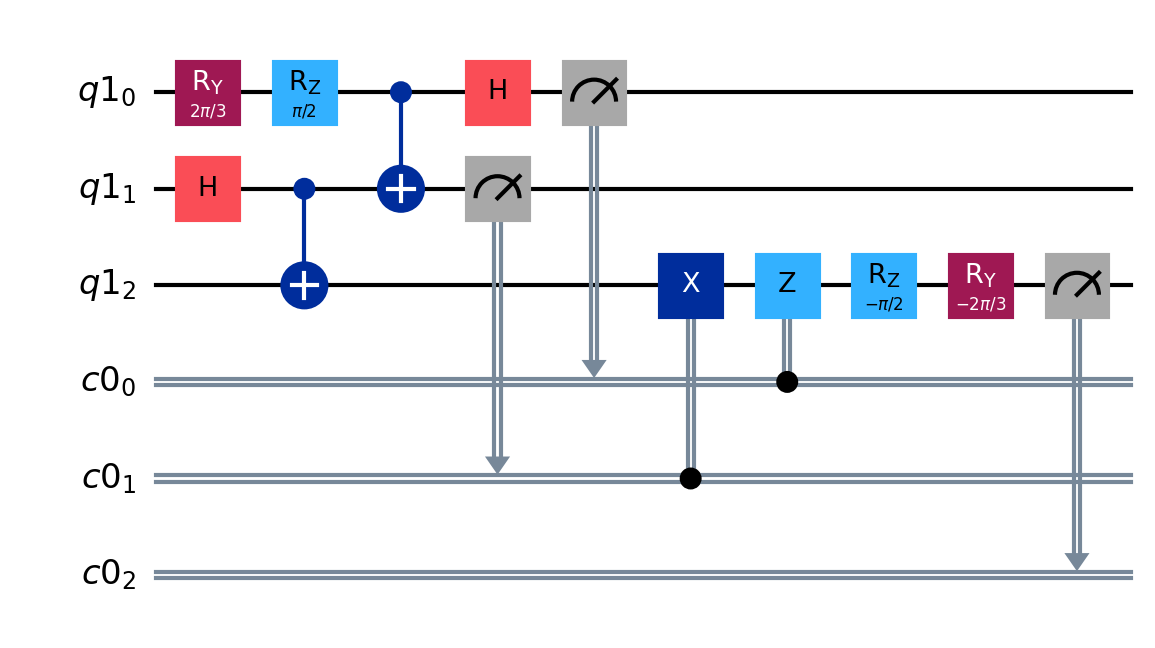
\includegraphics[width=0.80\textwidth]{images/homework3_q1_2pi3_pi2_aer.png}
\caption{Quantum teleportation}
\label{fig:homework3_q1_2pi3_pi2_aer}
\end{figure}

By default the program uses the AER simulator, which produces exact results according to the theory of quantum mechanics.
The program also accepts a \texttt{---provider} option to simulate the circuit using the noise models of IBM's quantum computers.

Some examples are:
\begin{lstlisting}[language=bash,basicstyle=\tiny]
bin/homework3_q1_qiskit.py --theta="pi/3" --phi="pi/2" --realign --provider=fake_sherbrooke
{0: 948, 1: 76}
bin/homework3_q1_qiskit.py --theta="pi/3" --phi="pi/2" --realign --provider=fake_osaka
{0: 949, 1: 75}
bin/homework3_q1_qiskit.py --theta="pi/3" --phi="pi/2" --realign --provider=fake_kyoto
{0: 512, 1: 512}
\end{lstlisting}
As we have seen before, the \texttt{fake\_kyoto} provider is not very good!
\end{enumerate}

I ran a range of values for $\theta$ and $\phi$ for several (fake) providers, and did contour plots of the accuracy,
shown in figure \ref{fig:homework3_q1_teleportation}.

\begin{figure}[htbp]
    \centering
    \captionsetup[subfigure]{labelformat=empty}
    \begin{subfigure}[b]{0.45\textwidth}
        \centering
        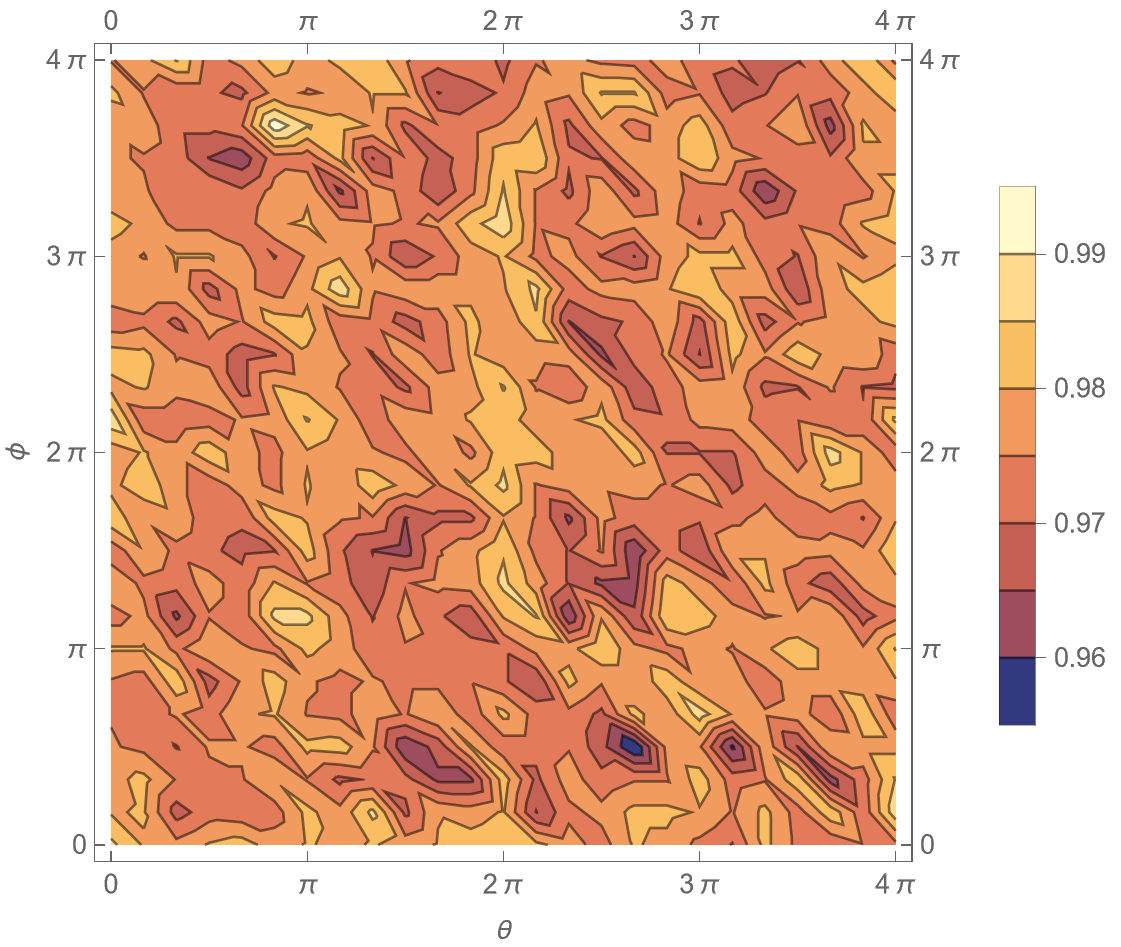
\includegraphics[width=\textwidth]{images/homework3_q1_algiers_contour.png}
        \caption{fake\_algiers}
    \end{subfigure}
    \hfill
    \begin{subfigure}[b]{0.45\textwidth}
        \centering
        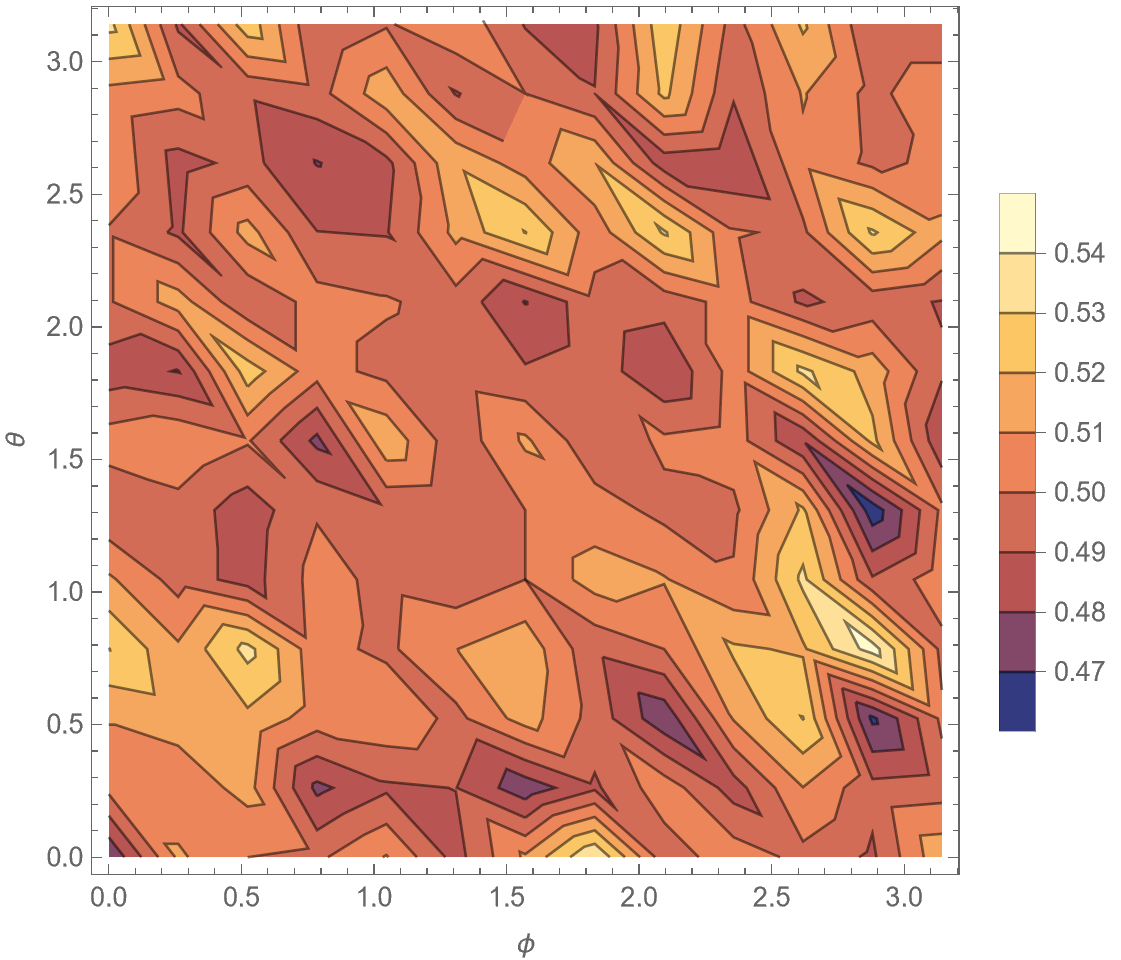
\includegraphics[width=\textwidth]{images/homework3_q1_kyoto_contour.png}
        \caption{fake\_kyoto}
    \end{subfigure}
    \vfill
    \begin{subfigure}[b]{0.45\textwidth}
        \centering
        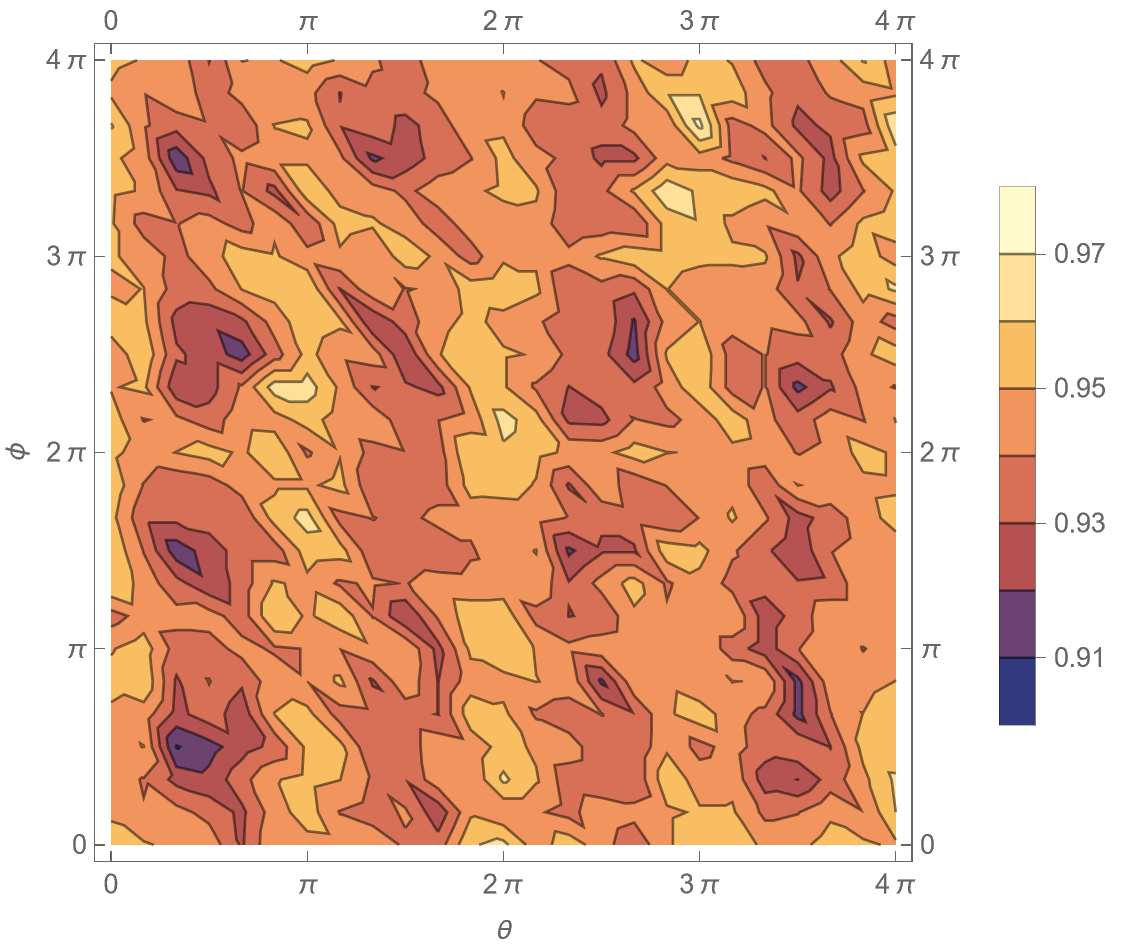
\includegraphics[width=\textwidth]{images/homework3_q1_osaka_contour.png}
        \caption{fake\_osaka}
    \end{subfigure}
    \hfill
    \begin{subfigure}[b]{0.45\textwidth}
        \centering
        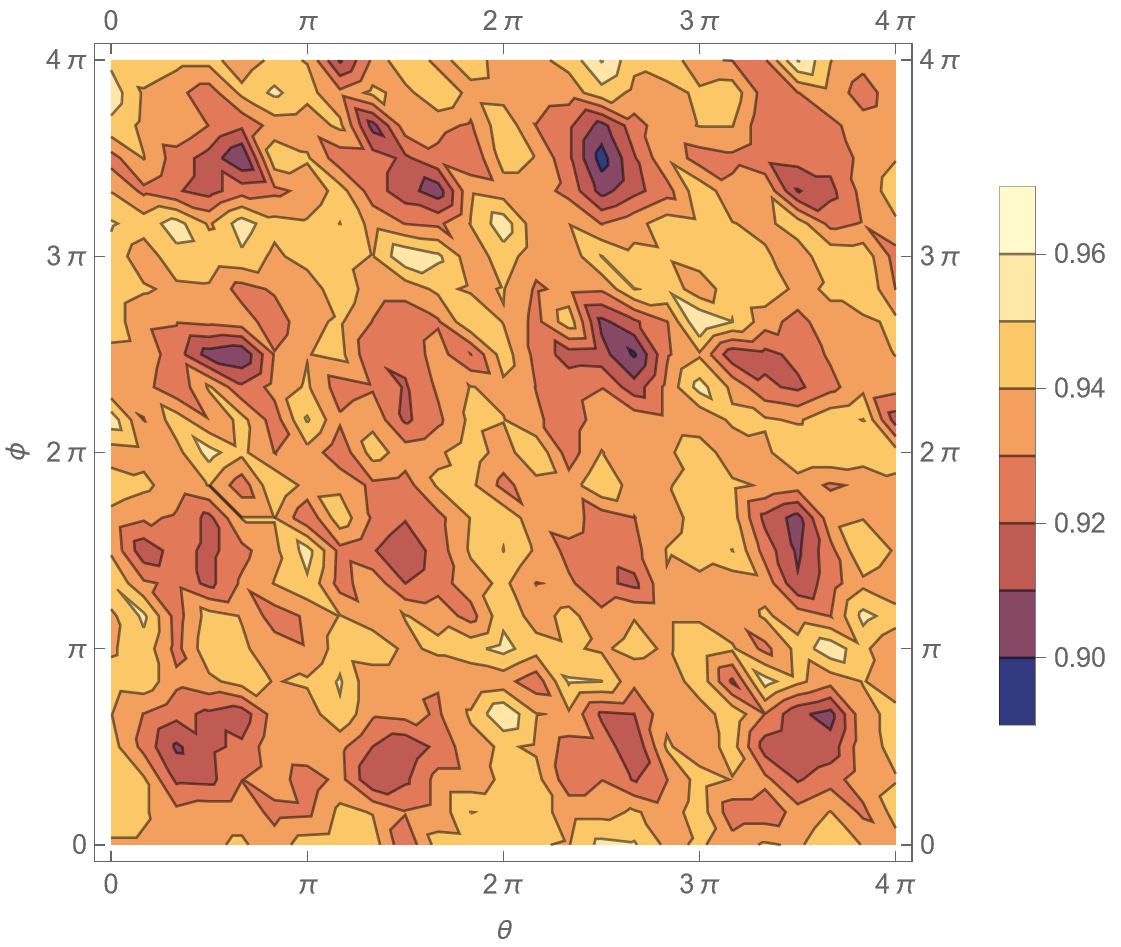
\includegraphics[width=\textwidth]{images/homework3_q1_sherbrooke_contour.png}
        \caption{fake\_sherbrooke}
    \end{subfigure}
    \caption{Quantum teleportation accuracy}
    \label{fig:homework3_q1_teleportation}
\end{figure}

It seems that for some providers at least, there may be a reduced accuracy in regions
where $\theta$ and $\phi$ are close to $k\pi+\pi/2$.
\texttt{fake\_osaka} and \texttt{fake\_sherbrooke} show a pretty clear periodic pattern.
With \texttt{fake\_kyoto} the acccuracy is so bad that we should probably ignore it.

%%%%%%%%%%%%%%%%%%%%%%%%%%%%%%%%%%%%%%%%%%%%%%%%%%%%%%%%%%%%%%%%%%%%%%%%%%%%%%%%%%%%%%%%%%%%%%%%%%%%
\newpage
\question{2}{Phase estimation: Example implementation (10 marks)

Implement the phase-estimation circuit to find the eigenvalue associated with eigenvector
\[
\ket{u} = \frac{1}{\sqrt{2}}\left(\ket{0} - i\ket{1}\right)
\]
of the unitary matrix
\[
\hat{U}_Y = \begin{pmatrix}
    1 & -i \\
    i & 1
\end{pmatrix}
\]
(\textit{Hint}: Two-bit precision will be enough for the purpose of this task!)
}

Wong\cite{wong2024} has a detailed worked example for two-qubit precision phase estimation for one of the eigenvalues of the Pauli Z matrix.
I adapted and generalised Wong's example into a QisKit program that does two-qubit phase estimation for either eigenvector of either of the Pauli Z or Pauli Y matrices.

The circuits generated by the program are shown in figure \ref{fig:homework3_q2_qpe}.

\begin{figure}[htbp]
    \centering
    \captionsetup[subfigure]{labelformat=empty}
    \begin{subfigure}[b]{0.45\textwidth}
        \centering
        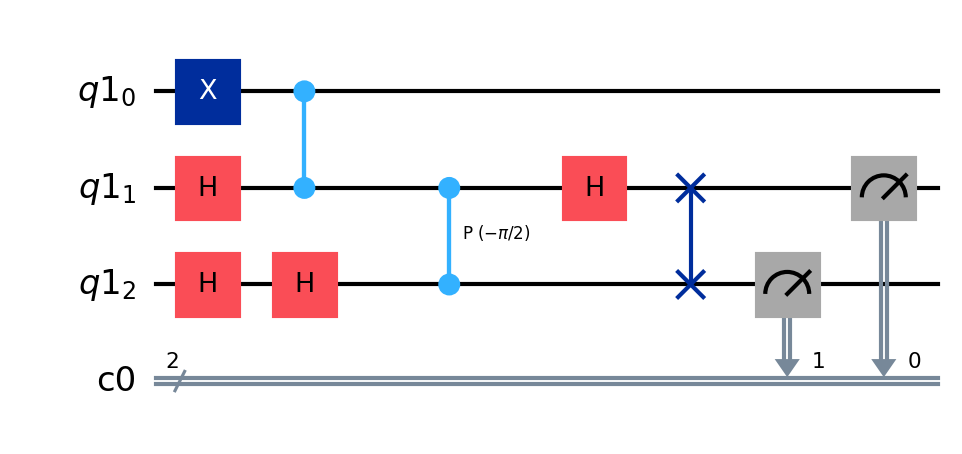
\includegraphics[width=\textwidth]{images/homework3_q2_qpe_z_e0.png}
        \caption{Operator Z, input $e_0=\begin{pmatrix} 0 \\ 1 \end{pmatrix}$}
    \end{subfigure}
    \hfill
    \begin{subfigure}[b]{0.45\textwidth}
        \centering
        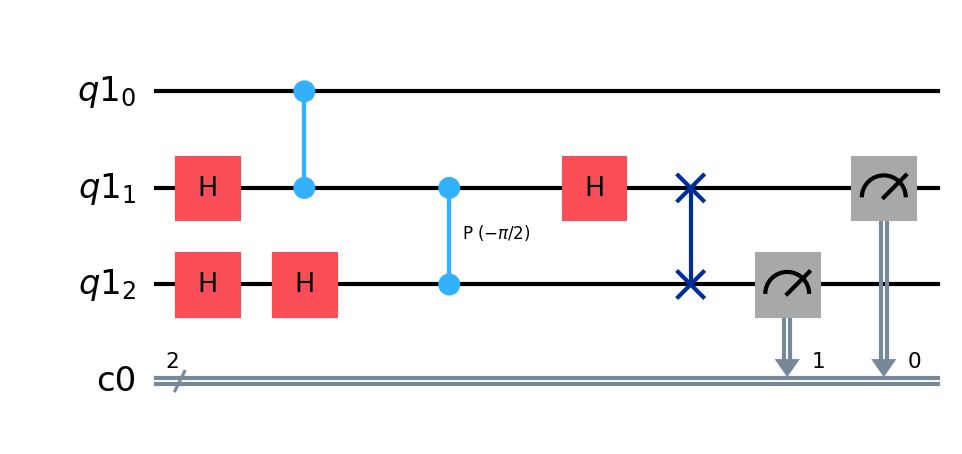
\includegraphics[width=\textwidth]{images/homework3_q2_qpe_z_e1.png}
        \caption{Operator Z, input $e_1=\begin{pmatrix} 1 \\ 0 \end{pmatrix}$}
    \end{subfigure}
    \vfill
    \begin{subfigure}[b]{0.45\textwidth}
        \centering
        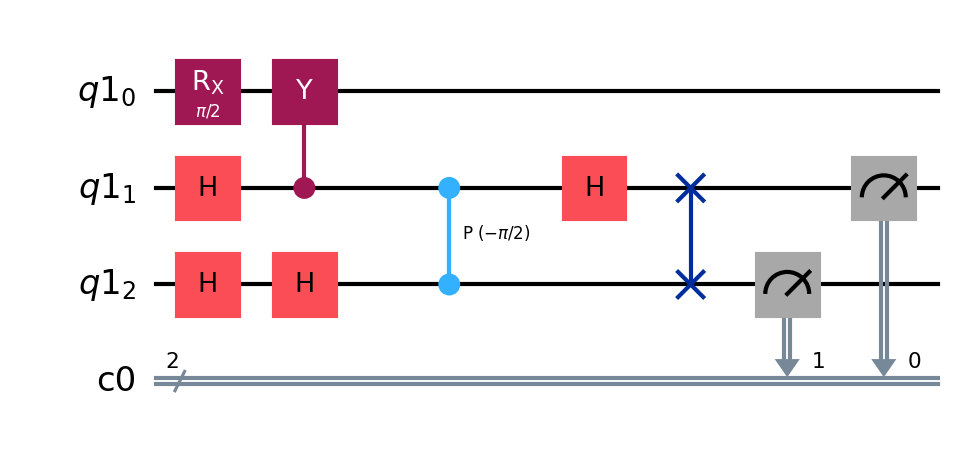
\includegraphics[width=\textwidth]{images/homework3_q2_qpe_y_e0.png}
        \caption{Operator Y, input $e_0=\frac{1}{\sqrt{2}}\begin{pmatrix} 1 \\ -i \end{pmatrix}$}
    \end{subfigure}
    \hfill
    \begin{subfigure}[b]{0.45\textwidth}
        \centering
        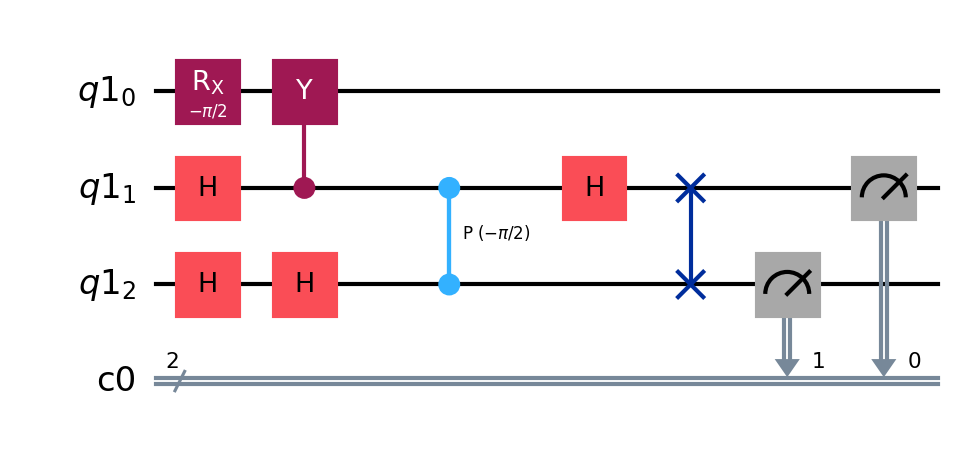
\includegraphics[width=\textwidth]{images/homework3_q2_qpe_y_e1.png}
        \caption{Operator Y, input $e_1=\frac{1}{\sqrt{2}}\begin{pmatrix} 1 \\ i \end{pmatrix}$}
    \end{subfigure}
    \caption{Quantum phase estimation}
    \label{fig:homework3_q2_qpe}
\end{figure}

The circuits vary in the state preparation of the input eigenvector,
and in the controlled unitary operator that is applied.

For the Z matrix the eigenvectors are
\begin{align*}
e_0 &= \begin{pmatrix} 0 \\ 1 \end{pmatrix} && \expl{Created with NOT gate}\\
e_1 &= \begin{pmatrix} 1 \\ 0 \end{pmatrix} && \expl{Created with identity gate}\\
\end{align*}
and the controlled unitary operator is the controlled Z gate.

For the Y matrix the eigenvectors are
\begin{align*}
e_0 &= \frac{1}{\sqrt{2}}\begin{pmatrix} 1 \\ -i \end{pmatrix} && \expl{Created with $R_X(\pi/2)$}\\
e_1 &= \frac{1}{\sqrt{2}}\begin{pmatrix} 1 \\ i \end{pmatrix} && \expl{Created with $R_X(-\pi/2)$}\\
\end{align*}

Running the program with the arguments for these setups yields the phases for the eigenvalues:

\begin{lstlisting}[language=bash]
bin/homework3_q2_qpe_simple_qiskit.py --operator=Z --eigenvector=e0
10: 1024
bin/homework3_q2_qpe_simple_qiskit.py --operator=Z --eigenvector=e1
00: 1024
bin/homework3_q2_qpe_simple_qiskit.py --operator=Y --eigenvector=e0
10: 1024
bin/homework3_q2_qpe_simple_qiskit.py --operator=Y --eigenvector=e1
00: 1024
\end{lstlisting}

For both matrices the eigenvalues are the same:
\begin{align*}
\lambda_0 &= -1 = e^{2i\pi\times \frac{1}{2}} && \expl{$k$=0.10 in binary}\\
\lambda_1 &= 1 = e^{2i\pi\times 0} && \expl{$k$=0.00 in binary}\\
\end{align*}

To explore phase estimation further, I wrote a more general program to do QPE for the $R_X(\theta)$ rotation gate.

For this gate, the eigenvalues and eigenvectors are:

\begin{align*}
\lambda_0 &= e^{-i\theta/2} & e_0 = \frac{1}{\sqrt{2}}\begin{pmatrix} 1 \\ 1 \end{pmatrix} && \expl{Created with $R_Y(\pi/2)$}\\
\lambda_1 &= e^{i\theta/2} & e_1 = \frac{1}{\sqrt{2}}\begin{pmatrix} -1 \\ 1 \end{pmatrix} && \expl{Created with $R_Y(-\pi/2)$}\\
\end{align*}

The program accepts the \texttt{---theta} argument to specify the angle $\theta$, and the \texttt{---bits} argument to specify the number of bits of precision.

Some examples are:

\begin{lstlisting}[language=bash,basicstyle=\tiny]
bin/homework3_q2_qpe_qiskit.py --operator=RX --eigenvector=e1 --bits=6 --theta="2*pi"
100000: 1024
bin/homework3_q2_qpe_qiskit.py --operator=RX --eigenvector=e1 --bits=6 --theta="pi"
010000: 1024
bin/homework3_q2_qpe_qiskit.py --operator=RX --eigenvector=e1 --bits=6 --theta="pi/2"
001000: 1024
bin/homework3_q2_qpe_qiskit.py --operator=RX --eigenvector=e1 --bits=6 --theta="pi/4"
000100: 1024
bin/homework3_q2_qpe_qiskit.py --operator=RX --eigenvector=e1 --bits=6 --theta="pi/8"
000010: 1024
bin/homework3_q2_qpe_qiskit.py --operator=RX --eigenvector=e1 --bits=6 --theta="pi/16"
000001: 1024
bin/homework3_q2_qpe_qiskit.py --operator=RX --eigenvector=e1 --bits=6 --theta="5*pi/16"
000101: 1024
bin/homework3_q2_qpe_qiskit.py --operator=RX --eigenvector=e1 --bits=6 --theta="21*pi/16"
010101: 1024
bin/homework3_q2_qpe_qiskit.py --operator=RX --eigenvector=e1 --bits=6 --theta="21*pi/8"
101010: 1024
\end{lstlisting}

The binary fractions shown correspond correctly to the phases of the eigenvalue for the $e_1$ eigenvector, for the specified values of $\theta$.
For example, with $\theta=2\pi$, the eigenvalue is $e^{i\pi}=e^{2i\pi\times\frac{1}{2}}$, so the binary fraction is 0.100000b.

Figure \ref{fig:qpe_rx_e1_21pi8} shows the circuit of the last command, with $\theta=21\pi/8$.
The program uses the QisKit circuit library QFT component, to simplify construction of the circuit with an arbitrary number of bits of precision.

\begin{figure}[H]
\centering
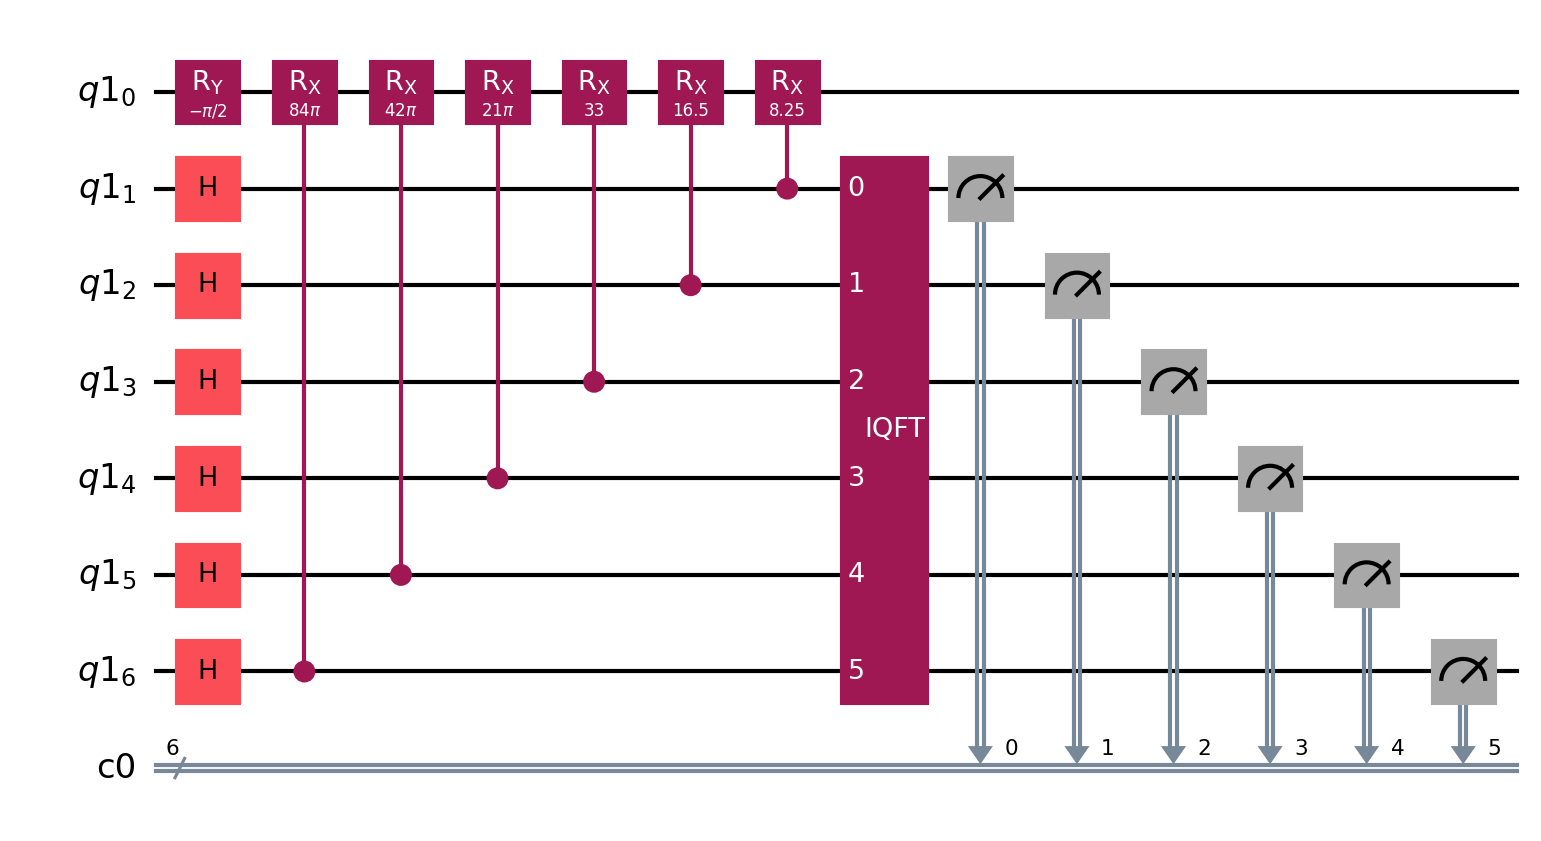
\includegraphics[width=0.80\textwidth]{images/homework3_q2_qpe_rx_e1_21pi8.png}
\caption{Quantum phase estimation with 6 bits of precision}
\label{fig:qpe_rx_e1_21pi8}
\end{figure}

Figure \ref{fig:qpe_rx_e1_21pi8_isa} shows the circuit, transpiled to the ISA architecture for the AER simulator.
(This expands the QFT component into its elementary gates.)

\begin{figure}[H]
\centering
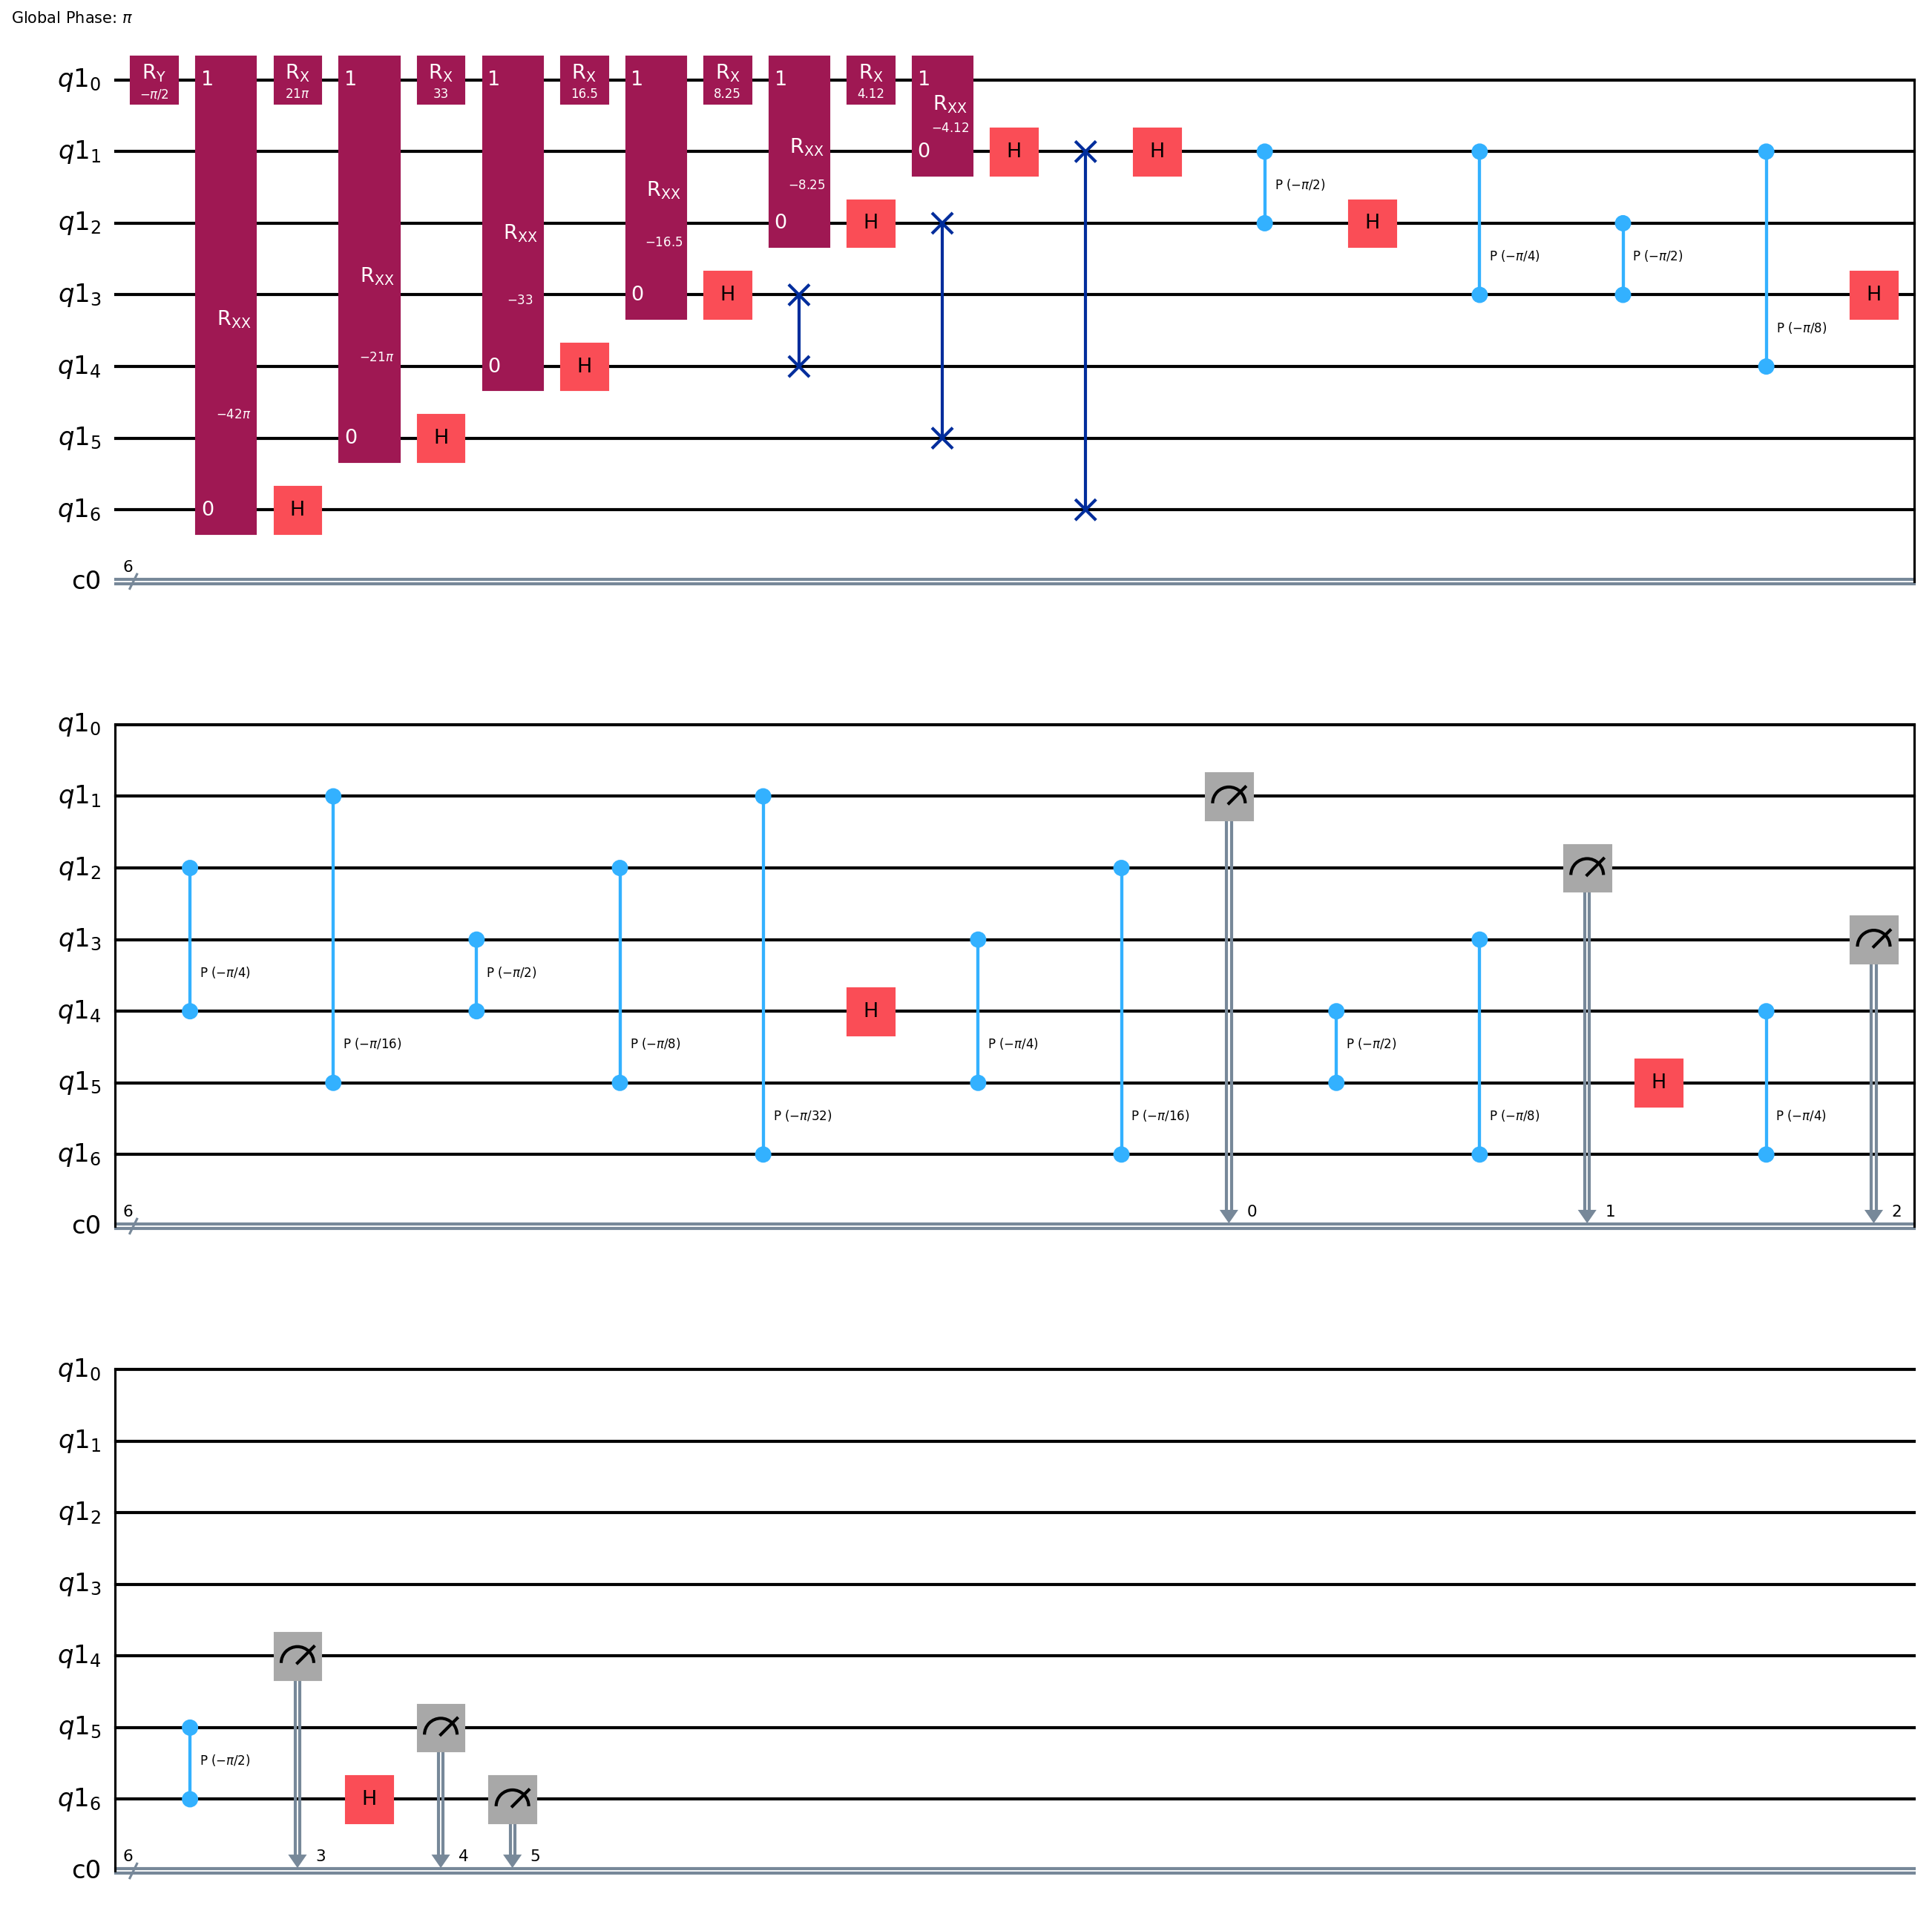
\includegraphics[width=0.80\textwidth]{images/homework3_q2_qpe_rx_e1_21pi8_isa.png}
\caption{Quantum phase estimation (ISA)}
\label{fig:qpe_rx_e1_21pi8_isa}
\end{figure}

This circuit gives perfect answers when $\theta$ has values that have a finite binary fractional expansion that fits within the specified number of bits.
When $\theta$ is some other value, the circuit gives a distribution of values.

As shown in the first command example above, when $\theta=2\pi$ the circuit gives the result 0.100000b with probability 1.
When we use $\theta=63\pi/32$, the correct phase is 0.1000001b, which falls halfway between two values that can be specified with 6 bits of precision.
We get this distribution:

\begin{lstlisting}[language=bash]
bin/homework3_q2_qpe_qiskit.py --operator=RX --eigenvector=e1 --bits=6 --theta="63*pi/32"
011111: 424
100011: 6
100000: 418
100001: 41
011110: 51
011101: 11
101010: 1
100100: 8
010110: 1
100010: 13
011010: 5
101100: 1
100101: 4
011100: 7
101101: 1
000010: 1
000100: 1
100110: 3
011000: 3
011011: 6
010111: 3
011001: 3
001000: 1
110000: 1
110111: 1
000001: 1
001011: 2
100111: 1
110011: 1
101000: 1
010010: 1
111100: 1
000111: 1
\end{lstlisting}

Most of the values are close to the correct value of 0.1000001b.
But there are a range of other values too.


%%%%%%%%%%%%%%%%%%%%%%%%%%%%%%%%%%%%%%%%%%%%%%%%%%%%%%%%%%%%%%%%%%%%%%%%%%%%%%%%%%%%%%%%%%%%%%%%%%%%
\newpage
\question{3}{Application: Quantum computational chemistry (5 bonus marks)

Inform yourself about the application of quantum algorithms (especially phase estimation)
in the context of quantum simulation of physical systems, especially quantum chemistry.
Use and resources at your disposal.
[A useful starting point could be reading some parts of the article S. McArdle et al.\cite{mcardle2020}]
Write a short summary (between $\frac{1}{2}$ and 1 page), discussing the main algorithmic ingredients and the quantum advantage.
}

This answer is mostly excerpts and summarisation of the paper by McArdle et al\cite{mcardle2020}.

Many problems in physical systems involve the analysis of Hamiltonians, in particular finding the ground state energy and the corresponding eigenvector.
A canonical problem is the \textit{electronic structure problem}, finding the quantum state of the electrons of an atom or molecule.
Beyond extremely simple systems, such problems are not amenable to analytic solutions; computational methods are used, hence the field of computational chemistry, for example.

Some of the problems belong to the bounded-error quantum polynomial time (BQP) complexity class,
which means that it is believed (though not yet proved) that the best classical or probabilistic algorithms have exponential running time,
but quantum algorithms have polynomial running time.

The Variational Quantum Eigensolver (VQE) is a hybrid quantum/classical algorithm that aims to find the lowest eigenvalue of a given Hamiltonian, such as that of a chemical system.
It is a promising near-term approach because it uses relatively few gates.

Quantum Phase Estimation (QPE) is a broadly-applicable quantum algorithm that can be used to find the lowest energy eigenstate and excited states of a physical Hamiltonian.
However, QPE requires circuits with a relatively large number of gates, and as such is of limited use for real-world problems until we can create fault-tolerant quantum computers with a larger number of qubits and gates.

Silva\cite{silva2024} includes a chapter on VQE using QisKit with some custom modules.
Hidary\cite{hidary2021} also discusses VQE, and includes an example of evolving an initial state under a Hamiltonian using Google's Circ and the OpenFermion library.


\printbibliography
\addcontentsline{toc}{section}{References}


\end{document}
